\documentclass[12pt,a4paper]{article}

\usepackage[utf8]{inputenc}
\usepackage[T2A]{fontenc}
\usepackage[ukrainian]{babel}
\usepackage{geometry}
\geometry{
    left=2cm,
    right=2cm,
    top=2cm,
    bottom=2cm
}

\usepackage[table]{xcolor}
\usepackage{amsmath}
\usepackage{graphicx}
\usepackage{subcaption}
\usepackage{multirow}
\usepackage{makecell}
\usepackage{pdflscape}
\usepackage{array}
\newcolumntype{C}[1]{>{\centering\arraybackslash}m{#1}}

\usepackage[
  unicode,
  pdftitle={ІО-41, Давидчук А.М., Цифрова схемотехніка, Лабораторна робота №1},
  pdfauthor={Давидчук Артем},
  pdfsubject={Цифрова схемотехніка}
]{hyperref}

\begin{document}

    \begin{titlepage}

        \begin{center}
\includegraphics[width=0.7\textwidth]{../../../TITLES/letterhead.png}\end{center}

        \begin{center}
            \large Національний технічний університет України\\
            «Київський політехнічний інститут імені Ігоря Сікорського»\\[1em]
            Факультет інформатики та обчислювальної техніки\\
            Кафедра обчислювальної техніки
        \end{center}

        \vfill

        \begin{center}
            \textbf{\LARGE Цифрова схемотехніка}\\[2em]
            \textbf{\Large Лабораторна робота №1}\\[0.5em]
            «Вивчення системи автоматизації проектування Quartus II. Синтез комбінаційних схем» 
        \end{center}

        \vfill

        \begin{flushright}
            Виконав: студент 2 курсу ФІОТ, гр. ІО-41\\
            \textit{Давидчук А. М.}\\
            Залікова книжка № 4106\\[1em]
            Перевірив: \textit{Нікольський С.\,С.}
        \end{flushright}

        \vfill

        \begin{center}Київ --- 2026\end{center}

    \end{titlepage}

    \noindent
    \textbf{\underline{Тема:}} «Вивчення системи автоматизації проектування Quartus II. Синтез комбінаційних схем».

    \vspace{1em}

    \noindent
    \textbf{\underline{Мета:}} Вивчення системи автоматизації проектування Quartus II. Отримання
    навичок створення проекту, вводу проекту в схемотехнічному режимі,
    роботи в графічному редакторі. Вивчення особливостей функціональної побудови суматорів. Розроблення
    функціональної схеми суматора в САПР Quartus II.

    \begin{center} \textbf{\large Хід роботи} \end{center}

    Мій номер залікової книжки: 4106, що у двіковому вигляді є 0001 0000 0000 1010.
    Звідси $h_7 = 0, h_6 = 0, h_5 = 0, h_4 = 1, h_3 = 0, h_2 = 1, h_1 = 0$.

    Звідси маю такий варіант:

    \begin{table}[h]
        \centering
        \renewcommand{\arraystretch}{1.3}
        \begin{tabular}{|cccccc|}
        \hline
        $0$ & $0$ & $1$ & $0$ & $1$ & $0$ \\
        \hline
        $h_6$ & $h_5$ & $h_4$ & $h_3$ & $h_2$ & $h_1$ \\
        \hline
        \end{tabular}
        \caption{Таблиця значеннь розрядів}
    \end{table}

    \noindent
    Параметри перемикальної функції:

    \begin{table}[h]
        \centering

        \begin{minipage}[t]{0.48\textwidth}
        \centering
        \renewcommand{\arraystretch}{1.2}
        \begin{tabular}{|c|c|}
        \hline
        $x_3\;\;x_2\;\;x_1$ & $f_4$ \\
        \hline
        $0\;\;0\;\;0$ & $0$ \\
        $0\;\;0\;\;1$ & $0$ \\
        $0\;\;1\;\;0$ & $0$ \\
        $0\;\;1\;\;1$ & $1$ \\
        $1\;\;0\;\;0$ & $0$ \\
        $1\;\;0\;\;1$ & $1$ \\
        $1\;\;1\;\;0$ & $0$ \\
        $1\;\;1\;\;1$ & $1$ \\
        \hline
        \end{tabular}
        \caption{Таблиця істинності функції $f_4$}
        \end{minipage}
        \hfill
        \begin{minipage}[t]{0.48\textwidth}
        \centering
        \renewcommand{\arraystretch}{1.4}
        \begin{tabular}{|c|c|}
        \hline
        \textbf{$h_1\;h_5\;h_2$} & \textbf{Логічні елементи} \\
        \hline
        $0\;0\;0$ & I-НЕ, I \\
        \hline
        \rowcolor{yellow!35}
        $0\;0\;1$ & I-НЕ \\
        \hline
        $0\;1\;0$ & АБО, I, НЕ \\
        \hline
        $0\;1\;1$ & I, АБО, НЕ \\
        \hline
        $1\;0\;0$ & АБО-НЕ, АБО \\
        \hline
        $1\;0\;1$ & I-НЕ, АБО \\
        \hline
        $1\;1\;0$ & АБО-НЕ, I-НЕ \\
        \hline
        $1\;1\;1$ & I, АБО-НЕ \\
        \hline
        \end{tabular}
        \caption{Елементний базис перемикальної функції}
        \end{minipage}

    \end{table}

    Звідси реалізую функцію $f_4$ у єдиному елементному базисі 2І-НЕ\slash 2І-НЕ (нехай використовуватиму саме 2І-НЕ елемент). 2І-НЕ\slash 2І-НЕ можна отримати із МДНФ функції $f_4$, додати два заперечення над усім виразом, а потім за законом де Моргана дійти до потрібної нормальної форми, а потім до операційної.

    \vspace{1em}

    ДДНФ функції $f_4$:

    \[
    f_4 (\text{ДДНФ}) = \overline{x_3} x_2 x_1 \vee x_3 \overline{x_2} x_1 \vee x_3 x_2 x_1
    \]

    \newpage

    І зробимо мінімізацію за допомогою діаграми Вейча:

    \begin{figure}[h]
        \centering
        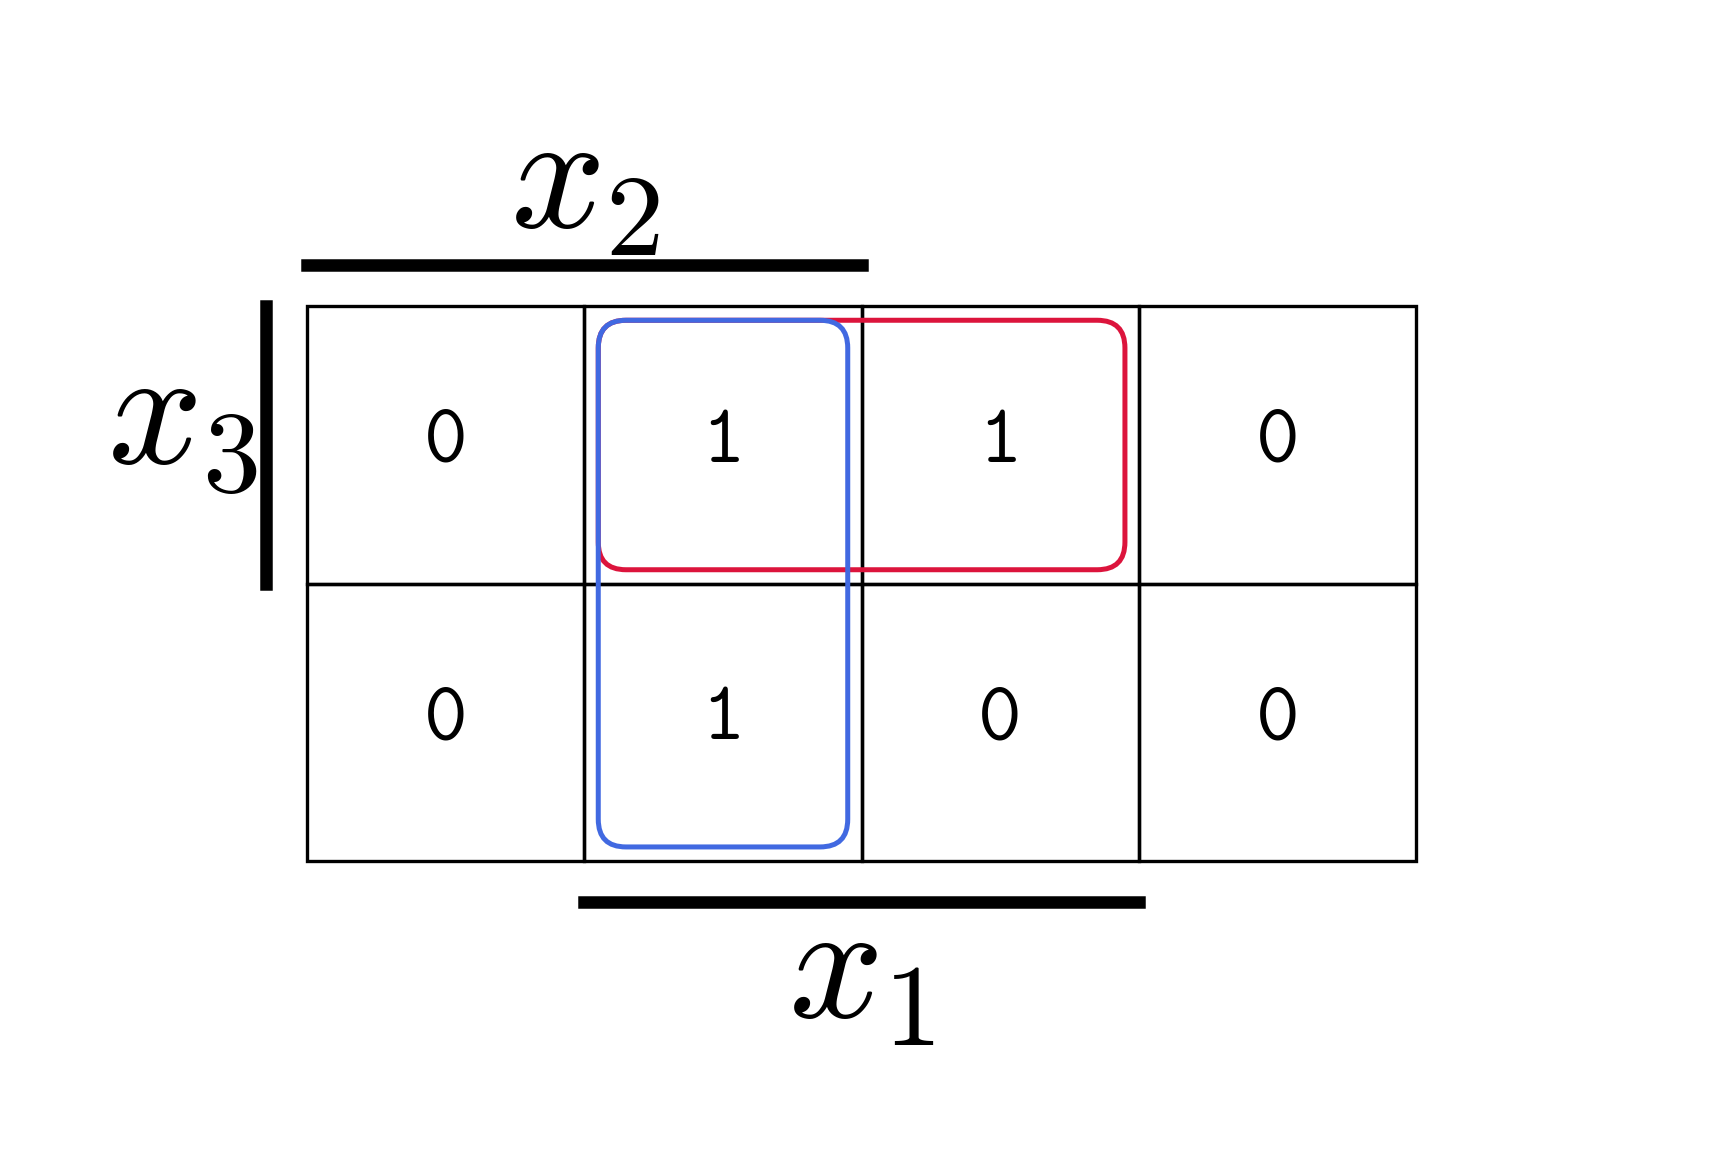
\includegraphics[width=0.5\textwidth]{media/minimized_f.png}
        \caption{Діаграма Вейча}
    \end{figure}

    \noindent
    Звідси МДНФ вираз для функції $f_4$:

    \vspace{0.5em}

    $f_4 (\text{МДНФ}) = x_2 x_1 \vee x_3 x_1$

    \vspace{1em}

    \noindent
    Тепер переведемо до нормальної форми:

    \vspace{0.5em}

    $f_4 (\text{МДНФ}) = \overline{\overline{f_4 (\text{МДНФ})}} = \overline{\overline{x_2 x_1 \vee x_3 x_1}} = \overline{\overline{x_2 x_1} \wedge \overline{x_3 x_1}}$

    \vspace{1em}

    \noindent
    А також визначимо операторну форму для елементів 2І-НЕ:

    \vspace{0.5em}

    $F_4 = \overline{\overline{x_2 x_1} \wedge \overline{x_3 x_1}}$

    \vspace{1em}

    \noindent
    Тепер побудуємо комбінаційну схему операторної функції $F_4$ у програмі Quartus II:

    \begin{figure}[h]
        \centering
        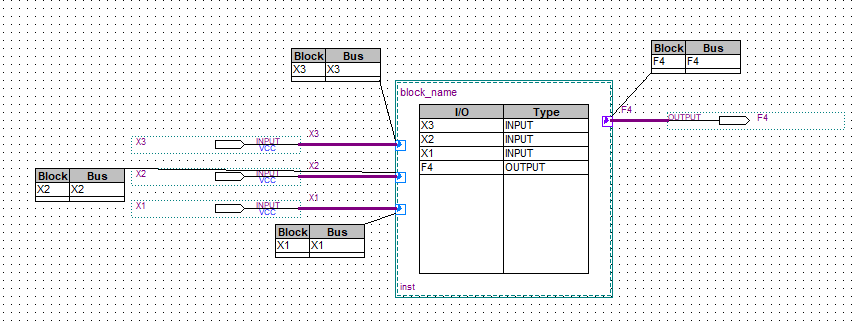
\includegraphics[width=\textwidth]{media/over_scheme.png}
        \caption{Загальна схема в програмі Quartus II}
    \end{figure}

    \newpage

    \noindent
    Схемна логіка блоку схеми:

    \begin{figure}[h]
        \centering
        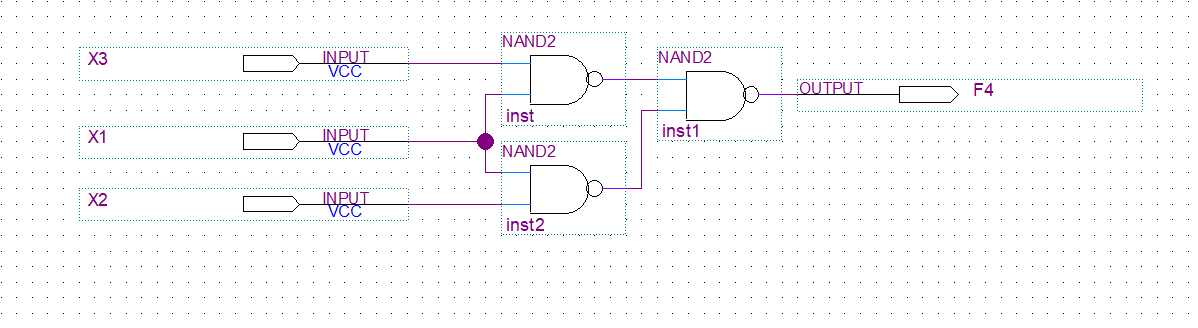
\includegraphics[width=\textwidth]{media/in_block_scheme.png}
        \caption{Операторне представлення функції $F_4$}
    \end{figure}

    \noindent
    Результат компіляції схеми:

    \begin{figure}[h]
        \centering
        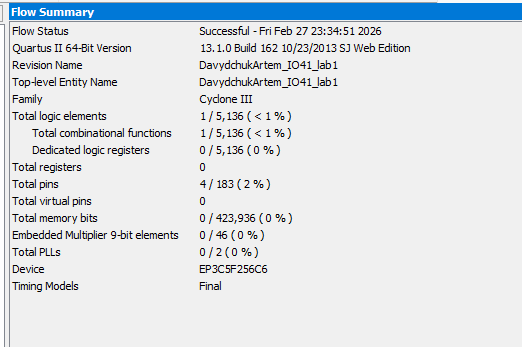
\includegraphics[width=0.7\textwidth]{media/compliation_summary.png}
        \caption{Операторне представлення функції $F_4$}
    \end{figure}

    \noindent
    Часова діаграма роботи схеми (перебираємо всі комбінації вхідних аргументів):

    \begin{figure}[h]
        \centering
        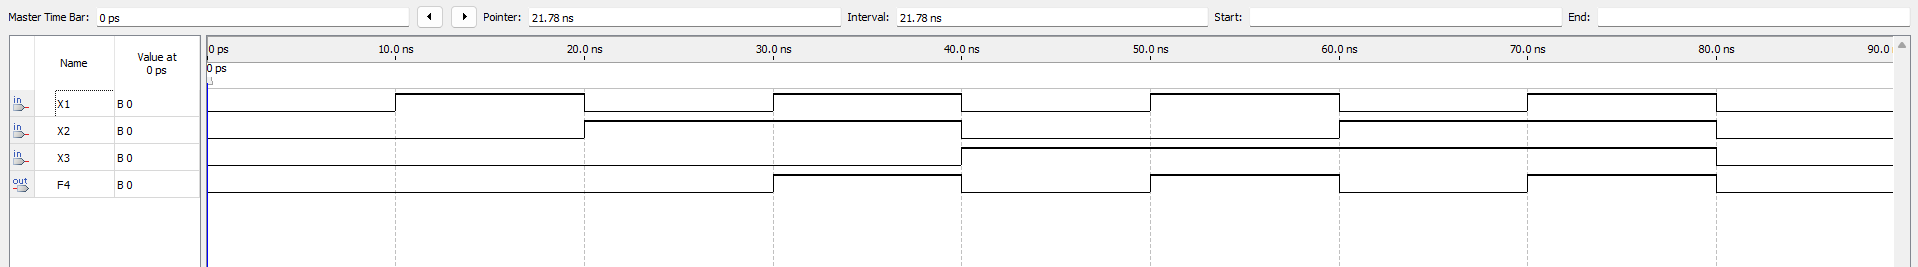
\includegraphics[width=0.8\textwidth]{media/timeline.png}
        \caption{Часова діаграма функції $F_4$}
    \end{figure}

    Як ми можемо бачити -- вихідний результат функції $F_4$ співпадає із тим, що у таблиці істинності.

    \newpage

    \begin{center} \textbf{\large Висновок} \end{center}

    У ході виконання лабораторної роботи було вивчено основні можливості САПР Quartus II та отримано практичні навички створення і налаштування проекту в графічному редакторі. За номером залікової книжки було визначено варіант завдання та задано параметри перемикальної функції $f_4$, після чого складено її таблицю істинності.

    Функцію $f_4$ було подано у ДДНФ та мінімізовано за допомогою діаграми Вейча, внаслідок чого отримано МДНФ:
    \[
    f_4 = x_2 x_1 \vee x_3 x_1.
    \]

    Далі виконано перетворення до форми, придатної для реалізації в єдиному елементному базисі 2І-НЕ, та отримано операторне представлення:
    \[
    F_4=\overline{\overline{x_2 x_1}\wedge \overline{x_3 x_1}}.
    \]

    На основі операторної форми було синтезовано комбінаційну схему в Quartus II, виконано компіляцію та моделювання. За результатами часової діаграми підтверджено, що вихідні значення $F_4$ для всіх комбінацій вхідних змінних співпадають з таблицею істинності, тобто синтезована схема реалізує задану логічну функцію коректно.

\end{document}